%%%%%%%% Does Closing the Modality Gap Help Hard-Negative-Trained CLIP?  (ICML-style paper) %%%%%%%%

\documentclass{article}

\usepackage{microtype}
\usepackage{graphicx}
\usepackage{subcaption}
\usepackage{booktabs}
\usepackage{hyperref}

\newcommand{\theHalgorithm}{\arabic{algorithm}}

\usepackage[preprint]{icml2026}
% no notice string in the first-page footnote
\makeatletter\renewcommand{\Notice@String}{}\makeatother

\usepackage{amsmath}
\usepackage{amssymb}
\usepackage{mathtools}
\usepackage{amsthm}
\usepackage{multirow}
\usepackage{array}
\usepackage{float}
\usepackage{placeins}
% allow more and larger floats per page so figures stay near their text
\renewcommand{\topfraction}{0.9}\renewcommand{\bottomfraction}{0.8}\renewcommand{\textfraction}{0.07}
\renewcommand{\floatpagefraction}{0.8}\renewcommand{\dbltopfraction}{0.9}\renewcommand{\dblfloatpagefraction}{0.8}
\setcounter{topnumber}{3}\setcounter{bottomnumber}{2}\setcounter{totalnumber}{5}\setcounter{dbltopnumber}{3}
\usepackage{xcolor}
\usepackage{tikz}
\usetikzlibrary{positioning,arrows.meta}
\usepackage[capitalize,noabbrev]{cleveref}

\newcommand{\uhat}{\hat{u}}
\newcommand{\gapnorm}{\lVert\Delta\rVert}

\icmltitlerunning{Does Closing the Modality Gap Help Hard-Negative-Trained CLIP?}

\begin{document}

\twocolumn[
  \icmltitle{Does Closing the Modality Gap Help Hard-Negative-Trained CLIP?}

  \begin{icmlauthorlist}
    \icmlauthor{Viren Mehta}{iitb}
    \icmlauthor{Shrey Patel}{iitb}
  \end{icmlauthorlist}

  \icmlaffiliation{iitb}{Indian Institute of Technology Bombay, Mumbai, India}

  \icmlkeywords{CLIP, modality gap, hard negatives, compositionality, NegCLIP}

  \vskip 0.3in
]

\printAffiliationsAndNotice{}

\begin{abstract}
The image and text embeddings of CLIP occupy two separate regions of the shared space, and removing this modality gap after training has been proposed as a way to make CLIP more robust at no cost in accuracy. We test this on CLIP models fine-tuned with hard negatives, the standard remedy for CLIP's weak compositional understanding. We fine-tune CLIP ViT-B/32 on COCO in five configurations, at three learning rates and with three seeds (30 runs), shift the embeddings in four ways, and evaluate retrieval, ARO and SugarCrepe with and without embedding noise. Closing the gap after training lowers retrieval for every model and lowers COCO-Order accuracy by up to 0.38 for models trained with hard captions; the loss is largest at the lowest learning rate, where fine-tuning barely moves the gap. We trace the whole effect to re-normalisation, which removes each caption's coordinate along the gap direction, a coordinate that hard-caption models use to rank a true caption above its negatives. A model fine-tuned with a penalty that closes the gap during training keeps or improves its compositional accuracy.
\end{abstract}

%=====================================================================
\section{Introduction}
\label{sec:intro}

CLIP \citep{radford2021clip} maps images and captions into a shared 512-dimensional space with two encoders trained by a contrastive loss. Although the loss rewards matched pairs for being close, the two modalities never mix: image embeddings and text embeddings occupy two narrow cones separated by a large offset, the \emph{modality gap} \citep{liang2022gap}. \citet{chowers2026bug} argue that this offset behaves like a constant vector orthogonal to how embeddings vary, and that removing it after training makes CLIP more robust to perturbations of the embeddings without changing clean accuracy.

A separate weakness of CLIP is that it behaves like a bag of words: it scores ``the horse is eating the grass'' and ``the grass is eating the horse'' almost equally \citep{yuksekgonul2023bow}. NegCLIP addresses this by fine-tuning on COCO with \emph{hard negative captions}, word-swapped versions of each caption, and \emph{hard negative images}, visually similar images, which raises word-order accuracy on COCO-Order from 0.46 to about 0.86.

Hard negative captions lie very close to the true caption in text space, so a post-hoc shift of the text embeddings could interact with exactly the fine distinctions that hard-negative training creates. We therefore ask: \textbf{does closing the modality gap help hard-negative-trained CLIP, and does hard-negative training change the gap?} We test three hypotheses:
\begin{itemize}
\item[\textbf{H1}] Hard-negative training changes the size of the gap.
\item[\textbf{H2}] As reported for CLIP, closing the gap improves robustness without hurting clean accuracy.
\item[\textbf{H3}] Image-to-text benchmarks compare captions of the same image, so a uniform shift of the text embeddings barely changes which caption wins.
\end{itemize}

Our contributions are:
\begin{itemize}
\item A grid of 30 fine-tuning runs that separates the effects of hard negative images, hard negative captions, batch size and learning rate on the gap and on compositional skill.
\item A post-hoc shift study over 8 models, 4 shift modes, 5 benchmarks and 4 noise levels, repeated on all 30 runs to measure the effect of the learning rate.
\item A mechanism: with re-normalisation, closing the gap removes each caption's coordinate along the gap direction, and hard-caption models use this coordinate. Removing random or high-variance directions instead costs almost nothing.
\item A test of closing the gap during training with a penalty on the distance between the modality means, which keeps or improves compositional accuracy.
\end{itemize}

%=====================================================================
\section{Related Work}
\label{sec:related}

\textbf{Contrastive learning.}
InfoNCE \citep{oord2018cpc} trains an encoder to pick the positive view of an input out of a set of negatives, and underlies SimCLR \citep{chen2020simclr} and CLIP. \citet{wang2020alignment} show that the loss optimises two properties: alignment of positive pairs and uniformity of the embeddings on the sphere. CLIP \citep{radford2021clip} applies InfoNCE across images and text with a learned temperature, and SigLIP \citep{zhai2023siglip} replaces the softmax with a pairwise sigmoid loss.

\textbf{The modality gap.}
\citet{liang2022gap} show that the gap is present at random initialisation, because each encoder maps its inputs into its own narrow cone, and that contrastive training preserves it; shifting the embeddings along the gap changes zero-shot accuracy and fairness. \citet{chowers2026bug} report that, when the gap is orthogonal to the embedding variation, closing it improves robustness to embedding perturbations at no clean cost. We test this claim on models trained for compositional understanding.

\textbf{Compositionality and hard negatives.}
The ARO benchmark \citep{yuksekgonul2023bow} tests relations, attributes and word order, and NegCLIP fine-tunes CLIP with hard negatives to solve it. SugarCrepe \citep{hsieh2023sugarcrepe} replaces ARO's often ungrammatical negatives with fluent ones, because a text-only model can solve many ARO cases. \citet{kamath2024hardpositive} show that hard-negative models can over-react to harmless rewordings of the true caption. Our work connects these lines of research: it measures how hard-negative training changes the gap, and how closing the gap changes compositional accuracy.

%=====================================================================
\section{Method}
\label{sec:method}

\subsection{Models and Fine-Tuning}

All models are OpenCLIP \citep{ilharco2021openclip} ViT-B/32 with QuickGELU activations, initialised from OpenAI CLIP.\footnote{The ARO code evaluates NegCLIP with standard GELU, which raises its COCO-Order score from 0.825 to 0.868 (\cref{app:sanity}).} Besides CLIP and the released NegCLIP checkpoint, we fine-tune five configurations on the NegCLIP training split of COCO \citep{lin2014coco} (\cref{tab:configs}). \emph{FT plain, batch 512} is a control: hard negative images double the number of images per batch, and this run separates a harder batch from a bigger one.

\begin{table}[t]
\caption{Fine-tuned configurations. img, cap: hard negative images and captions are used. The last column is the number of images per batch.}
\label{tab:configs}
\begin{center}
\begin{small}
\begin{tabular}{lccc}
\toprule
Configuration & img & cap & images/batch \\
\midrule
FT plain & & & 256 \\
FT plain, batch 512 & & & 512 \\
FT + hard captions & & $\checkmark$ & 256 \\
FT + hard images & $\checkmark$ & & 512 \\
FT NegCLIP recipe & $\checkmark$ & $\checkmark$ & 512 \\
\bottomrule
\end{tabular}
\end{small}
\end{center}
\vskip -0.1in
\end{table}

We re-implemented the NegCLIP training code in a single script. A batch of $N{=}256$ items holds the images $[I, I_{\text{hard}}]$ and the texts $[T, T(I_{\text{hard}}), T_{\text{neg}}, T_{\text{neg}}(I_{\text{hard}})]$, and the loss is
\begin{equation}
\mathcal{L} = \tfrac{1}{2}\big[\mathrm{CE}(\text{img}\times\text{all texts}) + \mathrm{CE}(\text{texts}_{1:|\text{img}|}\times\text{img})\big],
\label{eq:loss}
\end{equation}
so negative captions compete only in the image-to-text direction. All runs use 5 epochs, AdamW \citep{loshchilov2019adamw} with weight decay 0.2, a cosine schedule with 50 warm-up steps and fp16 mixed precision. Each configuration is trained at learning rates $\{10^{-5}, 5{\times}10^{-6}, 10^{-6}\}$ with seed 0, and the four main configurations again at $5{\times}10^{-6}$ and $10^{-6}$ with seeds 1 and 2. This gives 30 runs; the batch-512 control was run at the two lower rates. After every epoch we record the validation gap and Recall@1. The selected checkpoint of each configuration is the learning rate with the best final validation Recall@1, as in the NegCLIP paper.

\subsection{Measuring the Gap}

For $L_2$-normalised image embeddings $x_i$ and text embeddings $y_i$ of $n$ matched pairs we use the gap vector of \citet{liang2022gap},
\begin{equation}
\Delta = \tfrac{1}{n}\textstyle\sum_i x_i - \tfrac{1}{n}\sum_i y_i, \qquad \uhat = \Delta/\gapnorm .
\end{equation}
We report the gap $\gapnorm$, the cosine between the two centroids, the fraction of each modality's variance along $\uhat$ (a random direction gets $1/512$) and the linear separability of the two modalities.

\subsection{Shifting the Gap}

$\Delta$ is fitted on COCO val and applied unchanged to every test set. With $\mathcal{N}(v)=v/\lVert v\rVert$ and shift strength $\alpha$ ($\alpha{=}1$ closes the gap before re-normalisation, $\alpha{<}0$ widens it) we use four modes:
\begin{align}
\textit{text:}\ \ & y' = \mathcal{N}(y+\alpha\Delta) \label{eq:text}\\
\textit{both:}\ \ & x' = \mathcal{N}(x-\tfrac{\alpha}{2}\Delta),\ y' = \mathcal{N}(y+\tfrac{\alpha}{2}\Delta) \\
\textit{norenorm:}\ \ & y' = y+\alpha\Delta \label{eq:norenorm}\\
\textit{orth:}\ \ & y' = \mathcal{N}\big(y - (y^\top\uhat - \overline{y^\top\uhat})\,\uhat + \alpha\Delta\big) \label{eq:orth}
\end{align}
\emph{norenorm} and \emph{orth} are controls. \emph{norenorm} adds the same constant $\alpha x^\top\Delta$ to the score of every caption of an image, so it cannot change any image-to-text ranking. \emph{orth} first removes each caption's own deviation along $\uhat$, which makes $\Delta$ exactly orthogonal to the text variation, the condition assumed by \citet{chowers2026bug}; at $\alpha{=}0$ it applies no shift and only removes that deviation. Besides an $\alpha$ sweep from $-0.5$ to $1$, we solve for $\alpha$ by bisection so that the remaining gap on COCO val equals 0.6, 0.4, 0.2 or 0.1, which compares models at equal remaining gap.

\subsection{Closing the Gap During Training}

To test whether a small gap is harmful in itself, we also fine-tune with a penalty on the distance between the modality means,
\begin{equation}
\mathcal{L}_{\lambda} = \mathcal{L} + \lambda\,\lVert \bar x - \bar y\rVert^2 ,
\label{eq:penalty}
\end{equation}
where $\bar x$ and $\bar y$ are the batch means of the image embeddings and of their matched captions (hard negative captions excluded). We use $\lambda\in\{1, 10\}$ at learning rate $5{\times}10^{-6}$.

\subsection{Evaluation}

We report COCO 5k image$\to$text and text$\to$image Recall@1 on the Karpathy test split \citep{karpathy2015splits}; ARO COCO-Order, VG-Relation and VG-Attribution \citep{yuksekgonul2023bow}, the latter two built on Visual Genome \citep{krishna2017vg} and scored by macro accuracy;\footnote{Mean of the per-relation or per-attribute accuracies, so frequent relations do not dominate.} and SugarCrepe \citep{hsieh2023sugarcrepe} per subset. For robustness, Gaussian noise of expected norm $\sigma\in\{0.25, 0.5, 1\}$ is added to both modalities after the shift and the embeddings are re-normalised (3 noise seeds). Every model is encoded once and all shifts run on cached embeddings. Data, implementation and compute are described in \cref{app:data,app:impl}.

%=====================================================================
\section{Results}
\label{sec:exp}

Our pipeline reproduces the published numbers we could check: CLIP's gap (0.832 vs 0.82), CLIP's COCO Recall@1 (0.502 vs 0.502), and our NegCLIP recipe matches the released checkpoint on all three ARO tasks to within 0.013 (\cref{app:sanity}).

\subsection{Hard-Negative Training and the Gap}

\begin{figure}[t]
\begin{center}
\centerline{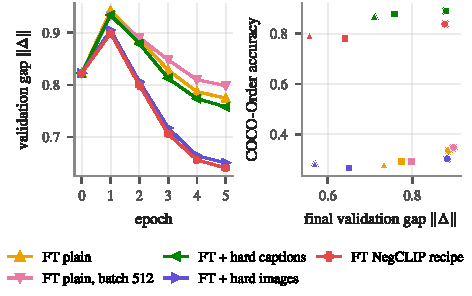
\includegraphics[width=\columnwidth]{figs/training_gap}}
\caption{Left: validation gap $\gapnorm$ (distance between the image and text centroids on COCO val) after each epoch, learning rate $5{\times}10^{-6}$. Right: COCO-Order accuracy (chance 0.2) against the final gap for every seed-0 run; marker shape gives the learning rate (circle $10^{-6}$, square $5{\times}10^{-6}$, triangle $10^{-5}$).}
\label{fig:training}
\end{center}
\vskip -0.2in
\end{figure}

\textbf{Hard negative images shrink the gap; batch size does not.}
Every run first widens the gap in epoch 1 (from 0.82 to 0.89--0.96) and then shrinks it (\cref{fig:training}, left). At $5{\times}10^{-6}$ the final gap is 0.650 with hard images and 0.640 with the NegCLIP recipe, against 0.775 for plain fine-tuning and 0.758 with hard captions; at $10^{-5}$ the order is the same (0.569 and 0.557 against 0.733 and 0.710). The batch-512 control ends at 0.799, so the larger batch does not explain the effect, and it stays within 0.015 of plain fine-tuning on every benchmark. At $10^{-6}$ all runs end near 0.88, so the learning rate sets how far the gap moves at all. In every model the gap direction holds only 0.2--0.4\% of the image variance and 0.7--0.8\% of the text variance, and the two modalities remain perfectly linearly separable (\cref{app:geometry}).

\begin{table}[t]
\caption{Clean accuracy at two learning rates (lr), mean $\pm$ std over 3 seeds (batch 512: one seed). C-Ord: COCO-Order accuracy (chance 0.2). VG-R, VG-A: VG-Relation and VG-Attribution macro accuracy (chance 0.5). R@1: COCO 5k image$\to$text Recall@1. NegCLIP (rel.): released checkpoint. Bold: best fine-tuned model per column and lr.}
\label{tab:matched}
\begin{center}
\begin{small}
\setlength{\tabcolsep}{2.6pt}
\begin{tabular}{llcccc}
\toprule
Model & lr & C-Ord & VG-R & VG-A & R@1 \\
\midrule
CLIP & -- & .472 & .638 & .632 & .502 \\
NegCLIP (rel.) & -- & .825 & .838 & .721 & .593 \\
\midrule
FT plain & 1e-6 & .333\tiny{$\pm$.005} & .591\tiny{$\pm$.002} & .650\tiny{$\pm$.002} & .614 \\
FT batch 512 & 1e-6 & .347 & .602 & .653 & .615 \\
FT + hard cap. & 1e-6 & \textbf{.890}\tiny{$\pm$.001} & \textbf{.856}\tiny{$\pm$.004} & \textbf{.729}\tiny{$\pm$.001} & .593 \\
FT + hard img. & 1e-6 & .301\tiny{$\pm$.001} & .553\tiny{$\pm$.003} & .648\tiny{$\pm$.001} & .607 \\
FT NegCLIP & 1e-6 & .838\tiny{$\pm$.001} & .841\tiny{$\pm$.004} & .724\tiny{$\pm$.002} & .595 \\
\midrule
FT plain & 5e-6 & .284\tiny{$\pm$.007} & .545\tiny{$\pm$.005} & .643\tiny{$\pm$.005} & .616 \\
FT batch 512 & 5e-6 & .292 & .556 & .643 & .623 \\
FT + hard cap. & 5e-6 & \textbf{.877}\tiny{$\pm$.002} & \textbf{.863}\tiny{$\pm$.005} & \textbf{.736}\tiny{$\pm$.004} & .601 \\
FT + hard img. & 5e-6 & .262\tiny{$\pm$.003} & .536\tiny{$\pm$.007} & .630\tiny{$\pm$.003} & .586 \\
FT NegCLIP & 5e-6 & .777\tiny{$\pm$.003} & .845\tiny{$\pm$.002} & .719\tiny{$\pm$.003} & .571 \\
\bottomrule
\end{tabular}
\end{small}
\end{center}
\vskip -0.15in
\end{table}

\textbf{Gap geometry.} \Cref{fig:app_geometry,tab:geometry} in \cref{app:geometry} describe the gap of the selected checkpoints on COCO test. Fine-tuning spreads the two modality centroids apart in angle (cosine 0.10--0.20, against 0.30 for CLIP) while the cosine of matched pairs stays at 0.29--0.30. The hard-image configurations were selected at $10^{-6}$, where the gap barely moves, which is why their selected checkpoints have the largest gaps here; \cref{tab:valgap} gives the comparison at matched learning rates.

\textbf{Compositional skill comes from hard captions.}
Only the two configurations with hard captions become compositional (\cref{tab:matched}). Hard captions alone give the best model at every learning rate, ahead of the released NegCLIP (COCO-Order 0.87--0.89 vs 0.825), and adding hard images to them lowers COCO-Order (0.890 to 0.838 at $10^{-6}$, 0.877 to 0.777 at $5{\times}10^{-6}$). Plain COCO fine-tuning improves retrieval but makes the model less order-sensitive than CLIP. The seed standard deviation is at most 0.007, 10--60 times smaller than the differences between configurations, and the ranking is the same at all three learning rates (\cref{app:train}). \Cref{fig:training} (right) puts these results together: runs with hard captions score 0.78--0.89 on COCO-Order at every gap from 0.56 to 0.88, and runs without them score 0.27--0.35 over the same range. \textbf{The size of the gap does not predict compositional skill}, and H1 holds for hard images but not for hard captions.

\subsection{Closing the Gap Post Hoc}

\begin{figure*}[t]
\begin{center}
\centerline{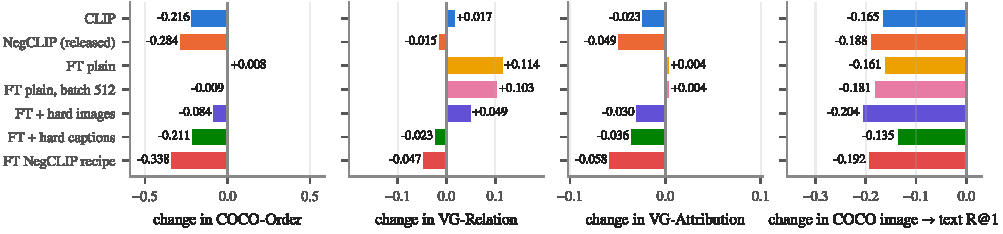
\includegraphics[width=\textwidth]{figs/closing_bars}}
\caption{Change in clean accuracy (shifted minus unshifted) when the text embeddings are moved along $\Delta$ until the remaining gap on COCO val is 0.10 (from 0.76--0.90). One bar per model, using the selected checkpoint of each configuration; negative values mean that closing the gap hurts.}
\label{fig:closing}
\end{center}
\vskip -0.2in
\end{figure*}

\Cref{fig:closing} shows the change in accuracy when the gap is closed to 0.10. For the selected checkpoints, every model trained with hard captions loses 0.21--0.34 on COCO-Order and 0.04--0.06 on VG-Attribution; our NegCLIP recipe falls from 0.838 to 0.500. Retrieval drops by 0.13--0.20 Recall@1 for every model. The only gains are on VG-Relation and only for models without hard captions (FT plain $+0.114$, batch 512 $+0.103$), which start well below CLIP there. The symmetric \emph{both} shift hurts more than the text shift (released NegCLIP COCO-Order $-0.387$ vs $-0.327$ at $\alpha{=}1$), mean and median gap vectors give results within 0.01 of each other, and widening the gap with the text shift changes accuracy by at most 0.02 (\cref{app:shift}). This rejects H2 on clean data.

\begin{figure*}[t]
\begin{center}
\centerline{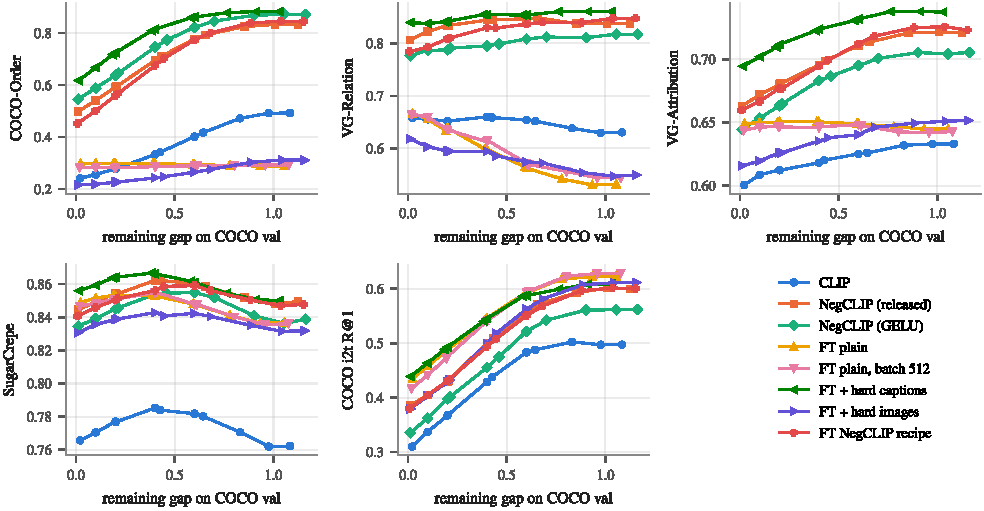
\includegraphics[width=\textwidth]{figs/app_shift_curves}}
\caption{Accuracy against the remaining gap on COCO val (text shift, mean $\Delta$, no noise). Points to the right of each model's original gap widen the gap ($\alpha<0$); moving left closes it.}
\label{fig:app_curves_shift}
\end{center}
\end{figure*}

\Cref{fig:app_curves_shift} shows the full text-shift curves. Accuracy changes smoothly with the remaining gap, and for the hard-caption models most of the COCO-Order loss happens below a remaining gap of 0.4.

\subsection{The Learning Rate Sets the Size of the Loss}

\begin{figure*}[t]
\begin{center}
\centerline{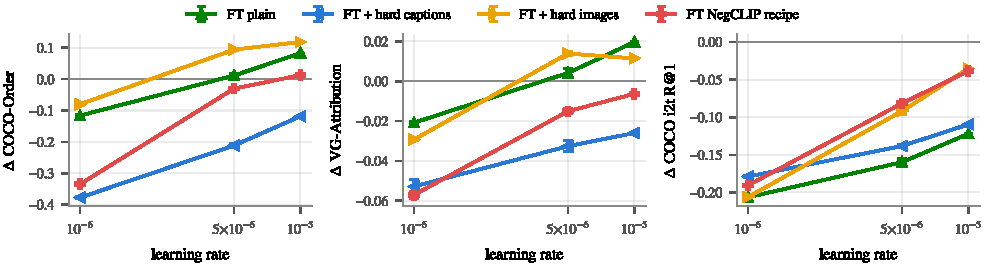
\includegraphics[width=\textwidth]{figs/lr_closing}}
\caption{Accuracy change (shifted minus unshifted) from closing the gap to 0.10 with the text shift, against the fine-tuning learning rate, for each configuration. Points: mean over seeds (3 at $10^{-6}$ and $5{\times}10^{-6}$, 1 at $10^{-5}$); error bars: std over seeds.}
\label{fig:lr}
\end{center}
\vskip -0.2in
\end{figure*}

The selected checkpoints come from different learning rates, so we repeated the shift on all 30 runs (\cref{fig:lr}, \cref{tab:lr} in \cref{app:lr}). The loss is largest at $10^{-6}$, where fine-tuning leaves the gap near 0.88: COCO-Order falls by 0.38 for FT + hard captions and 0.34 for the NegCLIP recipe, and Recall@1 by 0.18--0.21 for every configuration. At $10^{-5}$, where the gap ends at 0.56--0.73, the loss is 0.12 for hard captions, the NegCLIP recipe changes by $+0.01$, and Recall@1 falls by only 0.04--0.12. The seed standard deviation of each change is at most 0.007. Removing only the deviation along $\uhat$ (\emph{orth}, $\alpha{=}0$) follows the same trend, from $-0.36$ to $-0.01$ for the NegCLIP recipe. The more fine-tuning shrinks the gap, the less the models depend on its direction; FT + hard captions is the only configuration that loses more than 0.1 on COCO-Order at every learning rate.

\subsection{Why Closing the Gap Hurts}

The \emph{norenorm} shift (\cref{eq:norenorm}) leaves every accuracy unchanged to four decimals for all 8 models, so any effect of the shift comes from re-normalisation. Write a caption as $y = y_\perp + (m+d)\,\uhat$, where $m$ is the mean projection of all captions on $\uhat$ and $d$ is the caption's own deviation. After the \emph{text} shift,
\begin{equation}
s'(x,y) = \frac{x^\top y + \alpha\,x^\top\Delta}{\sqrt{1 + 2\alpha\gapnorm(m+d) + \alpha^2\gapnorm^2}} .
\label{eq:score}
\end{equation}
The numerator gains a constant that is shared by all captions of an image, and the denominator differs between captions only through $d$. Closing the gap therefore re-weights captions by their position along $\uhat$, and as the denominator grows the shifted score loses the information in $d$.

\begin{figure}[t]
\begin{center}
\centerline{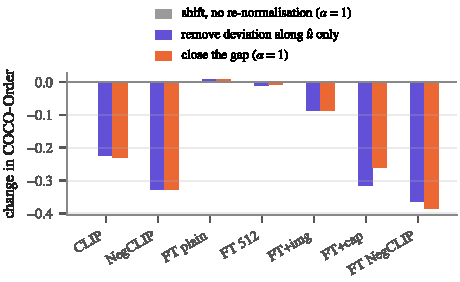
\includegraphics[width=\columnwidth]{figs/mechanism}}
\caption{Change in COCO-Order from three interventions for each model: the shift without re-normalisation (\emph{norenorm}, $\alpha{=}1$) is zero, and removing only $d$ (\emph{orth}, $\alpha{=}0$) matches closing the gap with re-normalisation (\emph{text}, $\alpha{=}1$).}
\label{fig:mech}
\end{center}
\vskip -0.25in
\end{figure}

The \emph{orth} control at $\alpha{=}0$ (\cref{eq:orth}) applies no shift and only removes $d$, and it reproduces the gap-closing change almost exactly (\cref{fig:mech}, \cref{tab:mechanism}): $-0.327$ vs $-0.327$ for released NegCLIP on COCO-Order, $-0.364$ vs $-0.385$ for our NegCLIP recipe, $-0.223$ vs $-0.231$ for CLIP, and $+0.143$ vs $+0.125$ for FT plain on VG-Relation. \textbf{Closing the gap amounts to deleting one direction from the text embeddings.} H3 holds only without re-normalisation.

\begin{table*}[t]
\caption{Removing each caption's deviation along $\uhat$ only (\emph{orth}, $\alpha=0$) against closing the gap (\emph{text}, $\alpha=1$).}
\label{tab:mechanism}
\begin{center}
\begin{small}
\begin{tabular}{lcccccc}
\toprule
& \multicolumn{2}{c}{COCO-Order} & \multicolumn{2}{c}{VG-Relation} & \multicolumn{2}{c}{VG-Attribution} \\
Model & remove $d$ & close gap & remove $d$ & close gap & remove $d$ & close gap \\
\midrule
CLIP & $-0.223$ & $-0.231$ & $+0.012$ & $+0.020$ & $-0.032$ & $-0.031$ \\
NegCLIP (released) & $-0.327$ & $-0.327$ & $-0.031$ & $-0.031$ & $-0.069$ & $-0.058$ \\
NegCLIP (GELU) & $-0.281$ & $-0.323$ & $-0.032$ & $-0.034$ & $-0.060$ & $-0.061$ \\
FT plain & $+0.008$ & $+0.007$ & $+0.143$ & $+0.125$ & $-0.001$ & $+0.002$ \\
FT plain, batch 512 & $-0.010$ & $-0.009$ & $+0.121$ & $+0.109$ & $-0.007$ & $+0.001$ \\
FT + hard captions & $-0.316$ & $-0.261$ & $-0.025$ & $-0.021$ & $-0.061$ & $-0.043$ \\
FT + hard images & $-0.086$ & $-0.087$ & $+0.061$ & $+0.064$ & $-0.036$ & $-0.034$ \\
FT NegCLIP recipe & $-0.364$ & $-0.385$ & $-0.052$ & $-0.056$ & $-0.071$ & $-0.065$ \\
\bottomrule
\end{tabular}
\end{small}
\end{center}
\end{table*}

\textbf{Is the gap direction special?}
The gap direction holds only about 0.7\% of the text variance, so it is nearly orthogonal to the text variation, yet removing the deviation along it costs CLIP and the hard-caption models 0.22--0.36 on COCO-Order. We compare it with two kinds of control directions (\cref{fig:x_removal}). Removing the deviation along any of 20 random unit directions changes accuracy by at most 0.019 on any benchmark. The top text principal component holds 4.3--5.8\% of the text variance, 6.6--7.7 times more than $\uhat$, yet removing it costs only 0.02--0.08 on COCO-Order; removing the top 5 components costs 0.06--0.17, still less than $\uhat$ alone for every hard-caption model.

\begin{figure*}[t]
\begin{center}
\centerline{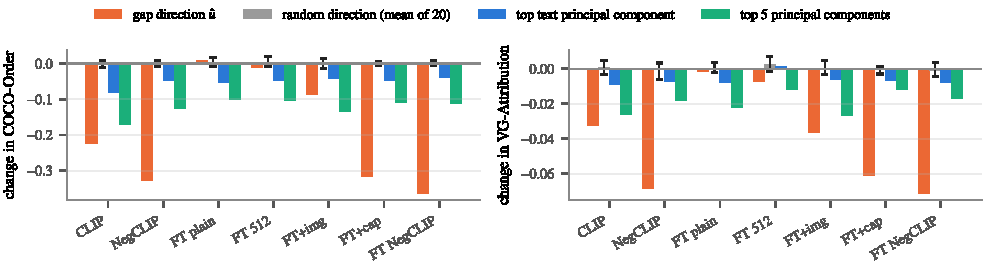
\includegraphics[width=\textwidth]{figs/x_direction_removal}}
\caption{Accuracy change from removing each caption's deviation from the benchmark mean along one direction or subspace: the gap direction $\uhat$, 20 random unit directions (bar: mean; whiskers: range) and the top 1 or 5 principal components of the COCO-val text embeddings.}
\label{fig:x_removal}
\end{center}
\vskip -0.2in
\end{figure*}

\textbf{The coordinate $d$ ranks captions.}
For released NegCLIP the true COCO-Order caption has the largest $d$ of the five options in 61\% of cases (chance 20\%). The probability that the true caption has a larger $d$ than a negative of the same case is 0.79--0.83 for hard-caption models, 0.68 for CLIP and 0.42 for FT plain (\cref{tab:x_auc}). Across all 32 model--benchmark pairs this probability predicts the effect of removing $d$ ($r=-0.88$, \cref{fig:probe}): where the true caption sits higher on $\uhat$, closing the gap hurts; where the negative does, as for FT plain on VG-Relation, it helps. The pairs whose sign disagrees all change by at most 0.01. The direction is not a naturalness direction: the Spearman correlation between $y^\top\uhat$ and GPT-2 \citep{radford2019gpt2} perplexity over 119,724 COCO-Order captions is between $-0.18$ and $+0.06$ for every model (\cref{app:nat}).

\begin{figure}[t]
\begin{center}
\centerline{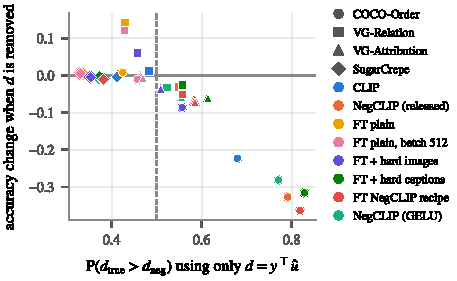
\includegraphics[width=\columnwidth]{figs/x_probe_vs_removal}}
\caption{One point per model and benchmark. x: fraction of (true, negative) caption pairs in which the true caption has the larger coordinate $d=y^\top\uhat$ along the gap direction (0.5, dashed: no information). y: accuracy change when $d$ is removed from every caption (\emph{orth}, $\alpha{=}0$). Pearson $r=-0.88$.}
\label{fig:probe}
\end{center}
\vskip -0.25in
\end{figure}

\textbf{Keeping $d$ does not prevent the loss.}
If the loss came only from deleting $d$, restoring it after the shift should prevent it. We close the gap with the text shift and then restore each caption's original deviation along $\uhat$, rescaled by the same factor as the rest of the vector. This recovers little (released NegCLIP COCO-Order 0.541 to 0.579, against 0.825 unshifted; \cref{tab:x_keep}), because every caption's score is still divided by its own norm $\lVert y+\alpha\Delta\rVert$ in \cref{eq:score}, which depends on $d$.

\subsection{SugarCrepe and Caption Length}

\begin{figure}[t]
\begin{center}
\centerline{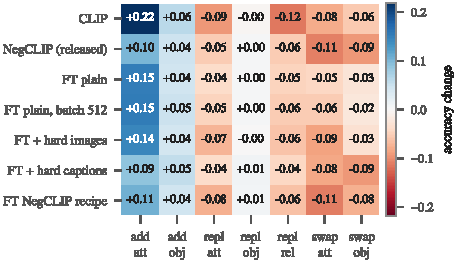
\includegraphics[width=\columnwidth]{figs/sugarcrepe_delta}}
\caption{Change in SugarCrepe accuracy per subset after closing the gap (text shift, $\alpha{=}1$). add/replace/swap: how the negative caption was built; att/obj/rel: the attribute, object or relation that was changed. Blue: gain; red: loss.}
\label{fig:sugarcrepe}
\end{center}
\vskip -0.25in
\end{figure}

Hard captions lift the SugarCrepe swap subsets (swap-att 0.70 to 0.78, swap-obj 0.67 to 0.78), and FT + hard captions has the best mean over subsets (0.837, released NegCLIP 0.829, CLIP 0.739; \cref{app:sugarcrepe}). Closing the gap helps add-att ($+0.09$ to $+0.22$) and add-obj ($+0.04$ to $+0.06$) and hurts the replace and swap subsets ($-0.03$ to $-0.11$), so the pooled score barely moves (\cref{fig:sugarcrepe}). The probe explains this pattern. The coordinate $d$ is weakly correlated with caption length (Spearman $\rho$ 0.09--0.20 on COCO-Order, 0.23--0.29 on SugarCrepe). In the add subsets the negative is on average 1.1 (add-att) and 3.3 (add-obj) words longer than the positive and has the larger $d$ in 76--98\% of cases, so removing $d$ removes a cue that favours the longer negative. Within a subset, however, the size of the length difference is only weakly related to the size of the $d$ difference ($\rho=0.06$--$0.19$), so length is one contributor rather than the full explanation.

\subsection{Robustness to Embedding Noise}

Under embedding noise the loss from closing the gap shrinks: for our NegCLIP recipe COCO-Order changes by $-0.338$ at $\sigma{=}0$, $-0.142$ at $\sigma{=}0.5$ and $-0.060$ at $\sigma{=}1$ (\cref{tab:noise}; \cref{fig:app_noise} in \cref{app:noise}). At $\sigma{=}0.5$ closing the gap gives every model $+0.03$ to $+0.05$ on SugarCrepe, and the gains of hard-negative models are no larger than those of CLIP (0.040) or FT plain (0.041). The benefit predicted by H2 thus appears only under noise and is not specific to hard-negative training.

\begin{table}[t]
\caption{Accuracy change from closing the gap to 0.10 when Gaussian noise of expected norm $\sigma$ is added to the image and text embeddings after the shift (mean of 3 noise seeds); $\sigma{=}0$ is the clean setting.}
\label{tab:noise}
\begin{center}
\begin{small}
\setlength{\tabcolsep}{2.4pt}
\begin{tabular}{lcccccc}
\toprule
& \multicolumn{3}{c}{COCO-Order} & \multicolumn{3}{c}{SugarCrepe} \\
Model & $\sigma{=}0$ & 0.5 & 1.0 & $\sigma{=}0$ & 0.5 & 1.0 \\
\midrule
CLIP & $-.216$ & $-.085$ & $-.034$ & $-.000$ & $+.040$ & $+.021$ \\
NegCLIP & $-.284$ & $-.124$ & $-.054$ & $-.003$ & $+.043$ & $+.022$ \\
FT plain & $+.008$ & $+.008$ & $+.002$ & $+.011$ & $+.041$ & $+.025$ \\
FT 512 & $-.009$ & $-.003$ & $-.003$ & $+.008$ & $+.048$ & $+.030$ \\
FT + cap. & $-.211$ & $-.136$ & $-.071$ & $+.005$ & $+.032$ & $+.021$ \\
FT + img. & $-.084$ & $-.030$ & $-.012$ & $+.001$ & $+.053$ & $+.027$ \\
FT NegCLIP & $-.338$ & $-.142$ & $-.060$ & $-.005$ & $+.045$ & $+.023$ \\
\bottomrule
\end{tabular}
\end{small}
\end{center}
\vskip -0.15in
\end{table}

\subsection{Closing the Gap During Training}

\begin{table}[t]
\caption{Fine-tuning with the penalty of \cref{eq:penalty} (lr $5{\times}10^{-6}$, seed 0; $\lambda{=}0$: no penalty). gap: final validation gap $\gapnorm$. Other columns as in \cref{tab:matched}.}
\label{tab:gapreg}
\begin{center}
\begin{small}
\setlength{\tabcolsep}{3.5pt}
\begin{tabular}{lcccccc}
\toprule
Config. & $\lambda$ & gap & C-Ord & VG-R & VG-A & R@1 \\
\midrule
FT + hard cap. & 0 & .758 & .878 & .860 & .738 & .599 \\
 & 1 & .038 & .907 & .852 & .732 & .587 \\
 & 10 & .030 & \textbf{.915} & \textbf{.867} & .727 & .583 \\
\midrule
FT NegCLIP & 0 & .640 & .781 & .847 & .723 & .574 \\
 & 10 & .033 & \textbf{.862} & .847 & .704 & .566 \\
\midrule
FT plain & 0 & .775 & .291 & .542 & .647 & .618 \\
 & 10 & .030 & .292 & \textbf{.610} & .631 & .599 \\
\bottomrule
\end{tabular}
\end{small}
\end{center}
\vskip -0.15in
\end{table}

\begin{figure}[t]
\begin{center}
\centerline{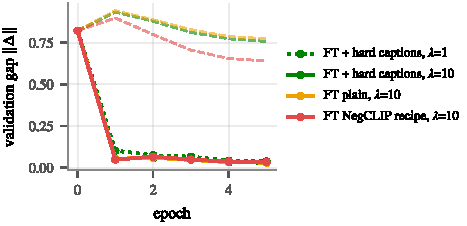
\includegraphics[width=\columnwidth]{figs/x_gapreg_curves}}
\caption{Validation gap during training with the gap penalty (solid and dotted) and without it (dashed, same configuration and learning rate).}
\label{fig:x_gapreg}
\end{center}
\end{figure}

If the loss comes from deleting a coordinate the model has learned to use, a model trained with a closed gap should not suffer. With the penalty of \cref{eq:penalty} the validation gap falls below 0.06 within one epoch and ends at 0.03--0.04 (\cref{tab:gapreg,fig:x_gapreg}). Compositional accuracy does not drop: COCO-Order rises from 0.878 to 0.915 with hard captions and from 0.781 to 0.862 with the NegCLIP recipe, and VG-Relation of FT plain rises from 0.542 to 0.610, at a cost of 0.01--0.02 Recall@1 and up to 0.02 on VG-Attribution. The COCO-Order gains are 5--10 times the seed standard deviation of \cref{tab:matched}. In these models removing $d$ changes COCO-Order by at most 0.009, so the compositional information no longer sits on the gap direction. The penalty does not improve robustness to noise: at $\sigma{=}0.5$, text$\to$image Recall@1 is 0.301 for FT + hard captions with $\lambda{=}10$ against 0.322 without it.

%=====================================================================
\FloatBarrier
\section{Discussion}
\label{sec:discussion}

The results separate two questions that are often treated as one: whether a model \emph{has} a small gap, and whether its gap is \emph{closed after training}. A small gap reached during training costs nothing: the penalty runs keep their compositional skill, and so do the high-learning-rate runs, whose gaps shrink to 0.56--0.71. Closing the gap after training is harmful in proportion to how much information the model stores along the gap direction, which the one-coordinate probe measures directly and which falls as the learning rate grows. The analysis behind \cref{eq:score} applies to any re-normalised shift of one modality, so the same check, the \emph{orth} control at $\alpha{=}0$ together with the probe, can be run on any CLIP-style model before its gap is closed.

%=====================================================================
\section{Conclusion}
\label{sec:conclusion}

Closing the modality gap after training does not help hard-negative-trained CLIP. At the selected learning rates it costs every model trained with hard captions 0.21--0.34 on COCO-Order and every model retrieval accuracy, and it helps only under strong embedding noise (H2 rejected). Re-normalisation turns the shift into the removal of each caption's coordinate along the gap direction, a coordinate that hard-caption models use to rank true captions above their negatives, while random and high-variance directions carry no such information (H3 rejected for order and attribute tasks). The loss shrinks as the learning rate grows, from 0.38 at $10^{-6}$ to at most 0.12 at $10^{-5}$. Hard negative images shrink the gap during training while hard negative captions give compositional skill (H1 partly supported), and a model trained with a penalty that keeps its gap near 0.03 keeps or improves its compositional accuracy.

%=====================================================================
\section*{Impact Statement}

This paper studies how a post-processing step for vision-language embeddings interacts with fine-tuning for compositional understanding. It uses public datasets and released models, and it introduces no new capability. We do not see societal consequences that need to be highlighted beyond those of CLIP-style models in general.

\bibliography{references}
\bibliographystyle{icml2026}

%=====================================================================
% APPENDIX
%=====================================================================
\newpage
\appendix
\onecolumn

\section{Data}
\label{app:data}

All data comes from MS-COCO \citep{lin2014coco} and Visual Genome \citep{krishna2017vg}. We split it so that no evaluation image was ever used for a gradient step (\cref{tab:data}).

\begin{table}[H]
\caption{Datasets and their roles. Chance accuracy is 0.2 for COCO-Order and 0.5 for the other compositional tasks.}
\label{tab:data}
\begin{center}
\begin{small}
\resizebox{\textwidth}{!}{\begin{tabular}{lll}
\toprule
Dataset & Size & Used for \\
\midrule
NegCLIP train split & 109,468 images & fine-tuning (1 caption, 1--6 hard negative captions and 3 neighbour images per row) \\
COCO Karpathy val & 5,000 images, 25,010 captions & checkpoint selection, per-epoch gap, fitting $\Delta$ \\
COCO Karpathy test & 5,000 images, 25,010 captions & gap measurement, retrieval Recall@1 \\
ARO COCO-Order & 25,010 cases & true caption vs 4 word-shuffled versions \\
ARO VG-Relation & 23,937 cases & true caption vs subject/object swap \\
ARO VG-Attribution & 28,748 cases & true caption vs attribute swap \\
SugarCrepe & 7,511 cases & fluent negatives: add (att 692, obj 2,062), replace (att 788, obj 1,652, rel 1,406), swap (att 666, obj 245) \\
GPT-2 (small) & 124M parameters & caption perplexity for the naturalness analysis \\
\bottomrule
\end{tabular}}
\end{small}
\end{center}
\end{table}

\textbf{Leakage check.} NegCLIP was trained on Karpathy train plus restval. We checked by file name that Karpathy val and test share no image with the NegCLIP training file. Karpathy val is NegCLIP's own validation set, so we use it only for checkpoint selection and for fitting $\Delta$, and report all results on Karpathy test, ARO and SugarCrepe.

\textbf{Fixed negatives.} The ARO code redraws the COCO-Order perturbations each time the data is loaded. We draw them once with seed 0 and cache them, so every model and every shift is scored on identical negatives.

\textbf{Download.} Evaluation needs only the 10,000 Karpathy val and test images. Instead of the full 6.2\,GB val2014 archive, we read the zip's central directory with HTTP range requests and fetched only those files (about 1.6\,GB). The 19\,GB of COCO 2014 images needed for fine-tuning were downloaded directly on the GPU server.

\section{Implementation and Compute}
\label{app:impl}

\textbf{Model loading.} OpenAI CLIP was trained with QuickGELU, and NegCLIP was fine-tuned from it, so every model is built as \texttt{ViT-B-32-quickgelu}. The released NegCLIP file is a 1.8\,GB training checkpoint with optimizer state; we extracted its 302 weight tensors with PyTorch's restricted loader.

\textbf{Training recipe.} 5 epochs; AdamW with $\beta=(0.9, 0.98)$, $\epsilon=10^{-6}$, weight decay 0.2 except on gains, biases and the logit scale; cosine schedule with 50 warm-up steps; fp16 mixed precision; learnable logit scale clamped at 100; RandomResizedCrop with scale 0.9--1.0. The batch is assembled as in \cref{eq:loss}, which gives logit matrices of $256{\times}256$ (FT plain), $512{\times}512$ (FT + hard images, batch 512), $256{\times}512$ (FT + hard captions) and $512{\times}1024$ (FT NegCLIP recipe). One hard negative caption and one neighbour image are drawn at random for each item in each epoch. The selected checkpoint of each configuration is the learning rate with the best final validation Recall@1, as in the NegCLIP paper ($5{\times}10^{-6}$ for FT plain and FT + hard captions, $10^{-6}$ for the others).

\textbf{Fast text encoding.} Captions are about 15 tokens long but padded to 77. CLIP's text encoder is causal and pools at the end-of-text token, so we run it only up to the longest caption in each batch. This gives the same embeddings (maximum difference $3{\times}10^{-7}$) at five times the speed on CPU.

\textbf{Pipeline.} \Cref{fig:pipeline} shows the pipeline. Every model is encoded once per benchmark; gap metrics, shifts, noise and evaluation then run on cached, normalised embeddings, so one shift setting takes seconds.

\begin{figure}[H]
\begin{center}
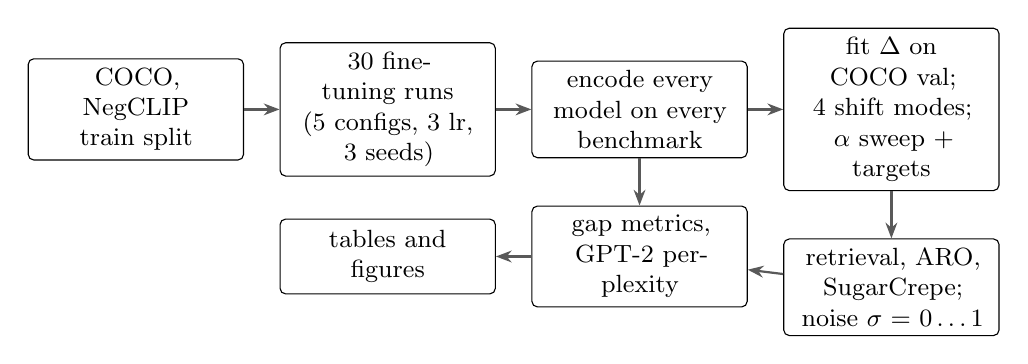
\begin{tikzpicture}[node distance=0.5cm and 0.45cm, every node/.style={font=\small},
  box/.style={draw, rounded corners=2pt, align=center, minimum height=0.95cm, text width=2.5cm},
  arr/.style={-{Stealth[length=2mm]}, thick, gray!70!black}]
\node[box] (data) {COCO, NegCLIP\\train split};
\node[box, right=of data] (ft) {30 fine-tuning runs\\(5 configs, 3 lr,\\3 seeds)};
\node[box, right=of ft] (enc) {encode every\\model on every\\benchmark};
\node[box, right=of enc] (shift) {fit $\Delta$ on COCO val;\\4 shift modes;\\$\alpha$ sweep + targets};
\node[box, below=0.6cm of shift] (eval) {retrieval, ARO,\\SugarCrepe;\\noise $\sigma=0\ldots1$};
\node[box, below=0.6cm of enc] (gap) {gap metrics,\\GPT-2 perplexity};
\node[box, left=of gap] (ana) {tables and\\figures};
\draw[arr] (data) -- (ft); \draw[arr] (ft) -- (enc); \draw[arr] (enc) -- (shift);
\draw[arr] (shift) -- (eval); \draw[arr] (enc) -- (gap); \draw[arr] (eval) -- (gap); \draw[arr] (gap) -- (ana);
\end{tikzpicture}
\caption{Experimental pipeline.}
\label{fig:pipeline}
\end{center}
\end{figure}

\textbf{Compute.} Development, CLIP and NegCLIP encoding, and the first shift sweeps ran on a 6-core laptop without a GPU. Fine-tuning and encoding of the 30 runs ran on a shared server with four 48\,GB GPUs. A scheduler launched a training job only when a GPU had enough free memory for it, so other users' jobs were never interrupted, and retried jobs that ran out of memory with a larger memory request. One epoch took a median of 219\,s (FT plain), 233\,s (batch 512), 266\,s (hard captions), 359\,s (hard images) and 411\,s (NegCLIP recipe); all 30 runs took about 16 GPU-hours. The 320 shift-evaluation tasks (8 models $\times$ 2 gap estimators $\times$ 4 modes $\times$ 5 benchmarks) ran on a 64-worker CPU pool with retries and timeouts. Clean scores of CLIP and NegCLIP from the server match the laptop run to within 0.0002.

\section{Sanity Checks}
\label{app:sanity}

\begin{table}[H]
\caption{Our numbers against published ones.}
\label{tab:sanity}
\begin{center}
\begin{small}
\resizebox{\textwidth}{!}{\begin{tabular}{lll}
\toprule
Check & Ours & Published \\
\midrule
CLIP gap $\gapnorm$ on COCO & 0.832 & 0.82 \citep{liang2022gap} \\
CLIP COCO 5k image$\to$text / text$\to$image R@1 & 0.502 / 0.302 & 0.502 / 0.304 \citep{radford2021clip} \\
CLIP VG-Relation / VG-Attribution / COCO-Order & 0.638 / 0.632 / 0.472 & 0.59--0.63 / 0.62 / 0.46 \citep{yuksekgonul2023bow} \\
Released NegCLIP VG-Relation / VG-Attribution / COCO-Order & 0.838 / 0.721 / 0.825 & 0.81 / 0.71 / 0.86 \citep{yuksekgonul2023bow} \\
Our NegCLIP recipe ($10^{-6}$) vs released NegCLIP & 0.840 / 0.725 / 0.838 & 0.838 / 0.721 / 0.825 \\
\bottomrule
\end{tabular}}
\end{small}
\end{center}
\end{table}

\textbf{An evaluation mismatch in the NegCLIP COCO-Order score.} NegCLIP was trained with QuickGELU, but the ARO repository evaluates it as a standard-GELU model. With the activation it was trained with, NegCLIP scores 0.825 on COCO-Order; with standard GELU it scores 0.868, which matches the paper's 0.86. The mismatch costs 2--3 points on VG-Relation, VG-Attribution and retrieval. We report the QuickGELU model throughout and keep the GELU version (``NegCLIP (GELU)'') as an extra reference.

\section{Training Dynamics, Matched Learning Rates and Seeds}
\label{app:train}

\begin{figure}[H]
\begin{center}
\centerline{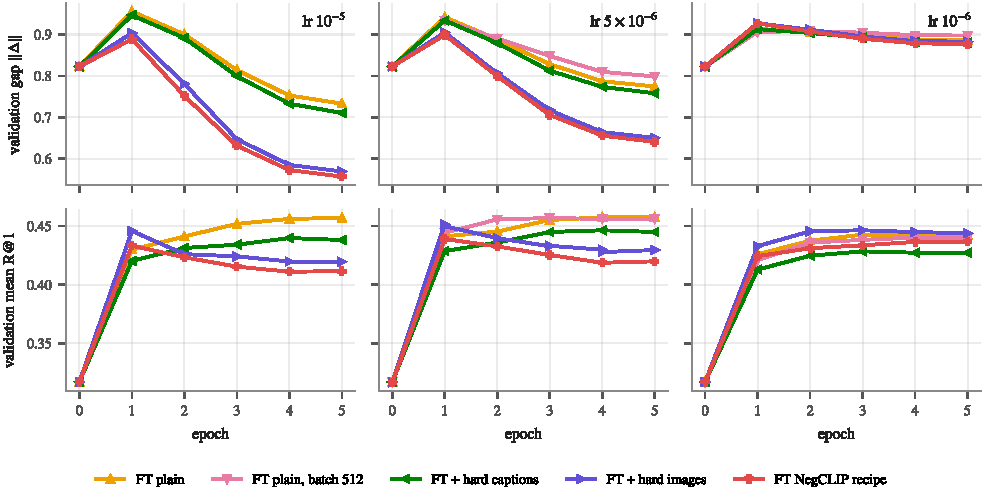
\includegraphics[width=\textwidth]{figs/app_training_curves}}
\caption{Validation gap (top) and validation mean Recall@1 (bottom) after each epoch, for every configuration and learning rate (seed 0).}
\label{fig:app_curves}
\end{center}
\end{figure}


\begin{table}[H]
\caption{Final-epoch validation gap and mean Recall@1 (seed 0). The batch-512 control was not run at $10^{-5}$.}
\label{tab:valgap}
\begin{center}
\begin{small}
\begin{tabular}{lcccccc}
\toprule
& \multicolumn{3}{c}{validation gap $\gapnorm$} & \multicolumn{3}{c}{validation mean R@1} \\
Configuration & $10^{-6}$ & $5{\times}10^{-6}$ & $10^{-5}$ & $10^{-6}$ & $5{\times}10^{-6}$ & $10^{-5}$ \\
\midrule
FT plain & 0.886 & 0.775 & 0.733 & 0.442 & 0.457 & 0.457 \\
FT plain, batch 512 & 0.897 & 0.799 & -- & 0.440 & 0.456 & -- \\
FT + hard captions & 0.880 & 0.758 & 0.710 & 0.427 & 0.445 & 0.438 \\
FT + hard images & 0.883 & 0.650 & 0.569 & 0.444 & 0.430 & 0.420 \\
FT NegCLIP recipe & 0.877 & 0.640 & 0.557 & 0.437 & 0.420 & 0.412 \\
\bottomrule
\end{tabular}
\end{small}
\end{center}
\end{table}

\begin{figure}[H]
\begin{center}
\centerline{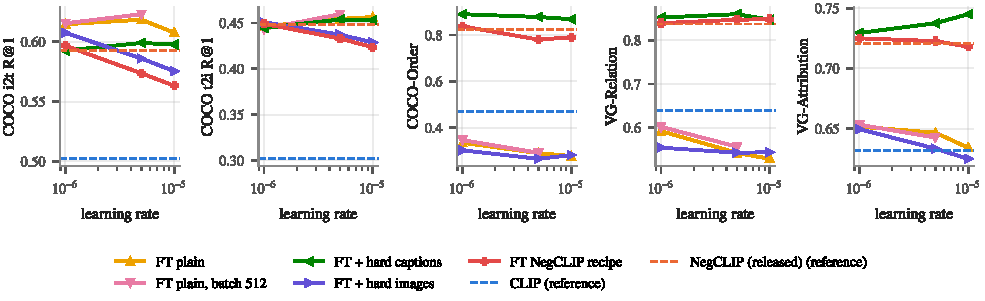
\includegraphics[width=\textwidth]{figs/app_matched_lr}}
\caption{Clean accuracy of every configuration at every learning rate (seed 0). Dashed lines: CLIP and released NegCLIP. The ranking of configurations is the same at every learning rate.}
\label{fig:app_mlr}
\end{center}
\end{figure}

\begin{table}[H]
\caption{Clean accuracy at learning rate $10^{-5}$ (seed 0), completing \cref{tab:matched}.}
\label{tab:lr1e5}
\begin{center}
\begin{small}
\begin{tabular}{lccccc}
\toprule
Configuration & i2t R@1 & t2i R@1 & COCO-Order & VG-Relation & VG-Attribution \\
\midrule
FT plain & 0.608 & 0.456 & 0.278 & 0.529 & 0.634 \\
FT + hard captions & 0.598 & 0.453 & \textbf{0.869} & 0.848 & \textbf{0.745} \\
FT + hard images & 0.575 & 0.429 & 0.282 & 0.544 & 0.625 \\
FT NegCLIP recipe & 0.563 & 0.423 & 0.791 & \textbf{0.849} & 0.718 \\
\bottomrule
\end{tabular}
\end{small}
\end{center}
\end{table}

\begin{figure}[H]
\begin{center}
\centerline{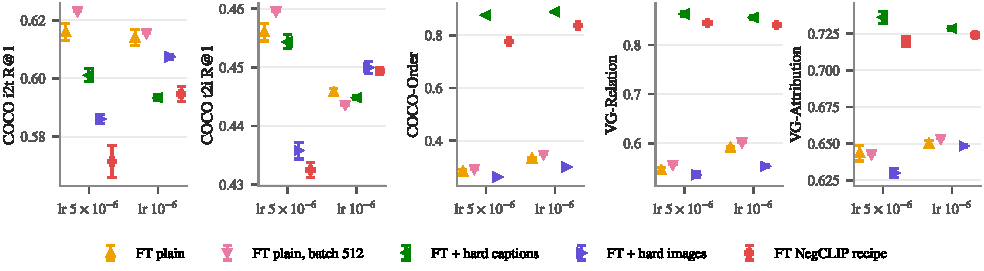
\includegraphics[width=\textwidth]{figs/app_seed_variance}}
\caption{Mean and standard deviation over seeds 0, 1 and 2. The error bars are barely visible because the standard deviation is at most 0.007.}
\label{fig:app_seeds}
\end{center}
\end{figure}

\textbf{Batch-size control.} At $5{\times}10^{-6}$ the batch-512 control ends with a gap of 0.799, against 0.775 for FT plain and 0.650 for FT + hard images; at $10^{-6}$ the three end at 0.897, 0.886 and 0.883. On the five clean metrics the control is within 0.015 of FT plain at both learning rates (\cref{tab:matched}). The gap reduction therefore comes from the hard negative images themselves, not from the number of images in the batch.

\section{Gap Geometry}
\label{app:geometry}

\begin{figure}[H]
\begin{center}
\centerline{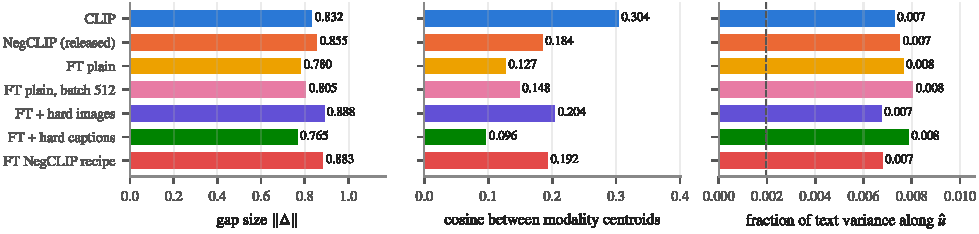
\includegraphics[width=\textwidth]{figs/app_gap_geometry}}
\caption{Gap geometry on COCO test for the selected checkpoint of each configuration. Right: fraction of text variance along $\uhat$; the dashed line is a random direction ($1/512$).}
\label{fig:app_geometry}
\end{center}
\end{figure}

\begin{table}[H]
\caption{Gap metrics on COCO test (selected checkpoints).}
\label{tab:geometry}
\begin{center}
\begin{small}
\resizebox{\textwidth}{!}{\begin{tabular}{lcccccc}
\toprule
Model & $\gapnorm$ & centroid cosine & matched-pair cosine & variance along $\uhat$ (img) & variance along $\uhat$ (text) & linear separability \\
\midrule
CLIP & 0.832 & 0.304 & 0.303 & 0.004 & 0.007 & 1.000 \\
NegCLIP (released) & 0.855 & 0.184 & 0.292 & 0.003 & 0.007 & 1.000 \\
NegCLIP (GELU) & 0.903 & 0.208 & 0.286 & 0.002 & 0.006 & 1.000 \\
FT plain & 0.780 & 0.127 & 0.297 & 0.003 & 0.008 & 1.000 \\
FT plain, batch 512 & 0.805 & 0.148 & 0.297 & 0.003 & 0.008 & 1.000 \\
FT + hard captions & 0.765 & 0.096 & 0.292 & 0.003 & 0.008 & 1.000 \\
FT + hard images & 0.888 & 0.204 & 0.297 & 0.002 & 0.007 & 1.000 \\
FT NegCLIP recipe & 0.883 & 0.192 & 0.293 & 0.002 & 0.007 & 1.000 \\
\bottomrule
\end{tabular}}
\end{small}
\end{center}
\end{table}



Image and text embeddings stay perfectly linearly separable in every model. The gap direction carries 0.2--0.4\% of the image variance and 0.7--0.8\% of the text variance, 3.5--4 times a random direction for text: nearly, but not exactly, orthogonal to the variation. Fine-tuning spreads the two modality centroids apart in angle (cosine 0.10--0.20 against 0.30 for CLIP). The hard-image configurations were selected at $10^{-6}$, where the gap barely moves, which is why their selected checkpoints have the largest gaps here; \cref{tab:valgap} gives the matched comparison.

\begin{figure}[H]
\begin{center}
\centerline{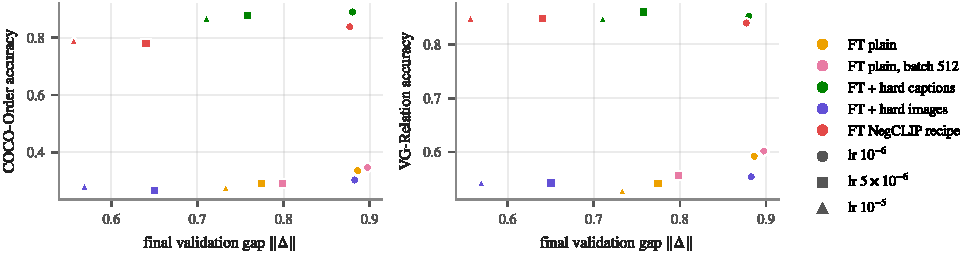
\includegraphics[width=0.85\textwidth]{figs/app_gap_vs_skill}}
\caption{Clean COCO-Order and VG-Relation accuracy against the final validation gap for every seed-0 run.}
\label{fig:app_gapskill}
\end{center}
\end{figure}

\section{Full Shift Results}
\label{app:shift}

\begin{table}[H]
\caption{Change in clean accuracy when the remaining gap on COCO val is reduced to 0.10 (text shift, mean $\Delta$).}
\label{tab:closing}
\begin{center}
\begin{small}
\begin{tabular}{lcccccc}
\toprule
Model & gap before & COCO-Order & VG-Relation & VG-Attribution & SugarCrepe & COCO i2t R@1 \\
\midrule
CLIP & 0.831 & $-0.216$ & $+0.017$ & $-0.023$ & $-0.000$ & $-0.165$ \\
NegCLIP (released) & 0.853 & $-0.284$ & $-0.015$ & $-0.049$ & $-0.003$ & $-0.188$ \\
NegCLIP (GELU) & 0.902 & $-0.279$ & $-0.024$ & $-0.052$ & $-0.002$ & $-0.199$ \\
FT plain & 0.779 & $+0.008$ & $+0.114$ & $+0.004$ & $+0.011$ & $-0.161$ \\
FT plain, batch 512 & 0.803 & $-0.009$ & $+0.103$ & $+0.004$ & $+0.008$ & $-0.181$ \\
FT + hard captions & 0.763 & $-0.211$ & $-0.023$ & $-0.036$ & $+0.005$ & $-0.135$ \\
FT + hard images & 0.886 & $-0.084$ & $+0.049$ & $-0.030$ & $+0.001$ & $-0.204$ \\
FT NegCLIP recipe & 0.881 & $-0.338$ & $-0.047$ & $-0.058$ & $-0.005$ & $-0.192$ \\
\bottomrule
\end{tabular}
\end{small}
\end{center}
\end{table}

\textbf{Shift settings.} For each model we ran 7 values of $\alpha$ and 4 target gaps, each with the mean and the coordinate-wise median gap vector, in all four modes. The two estimators give results within 0.01 of each other. The symmetric \emph{both} shift is consistently more harmful than the text shift. Widening the gap ($\alpha<0$) changes accuracy by at most 0.02 with the text shift; with the symmetric shift the largest changes are $-0.108$ in CLIP image$\to$text Recall@1 and $+0.081$ in CLIP COCO-Order at $\alpha=-0.5$. Pooled SugarCrepe accuracy peaks slightly ($+0.01$ to $+0.02$) at a remaining gap near 0.4 and returns to its starting value at 0.1; \cref{app:sugarcrepe} shows the large opposite changes between subsets behind this.

\section{Mechanism Details}
\label{app:mechanism}

\begin{figure}[H]
\begin{center}
\centerline{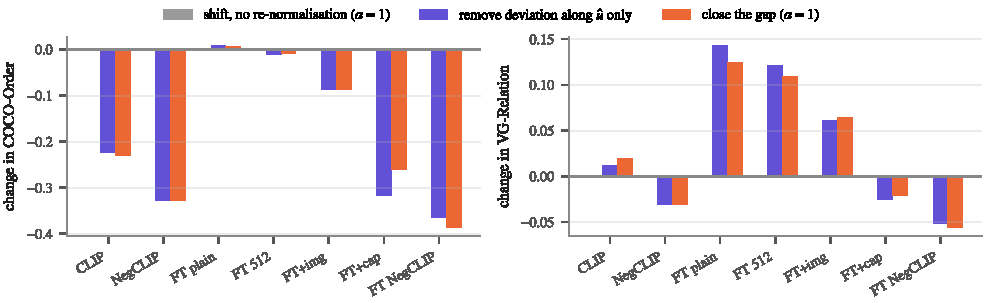
\includegraphics[width=\textwidth]{figs/app_mechanism}}
\caption{Change in COCO-Order and VG-Relation from three interventions: the shift without re-normalisation (grey) is exactly zero for every model, and removing each caption's deviation along $\uhat$ alone (purple) matches closing the gap (orange).}
\label{fig:app_mech}
\end{center}
\end{figure}

\begin{figure}[H]
\begin{center}
\centerline{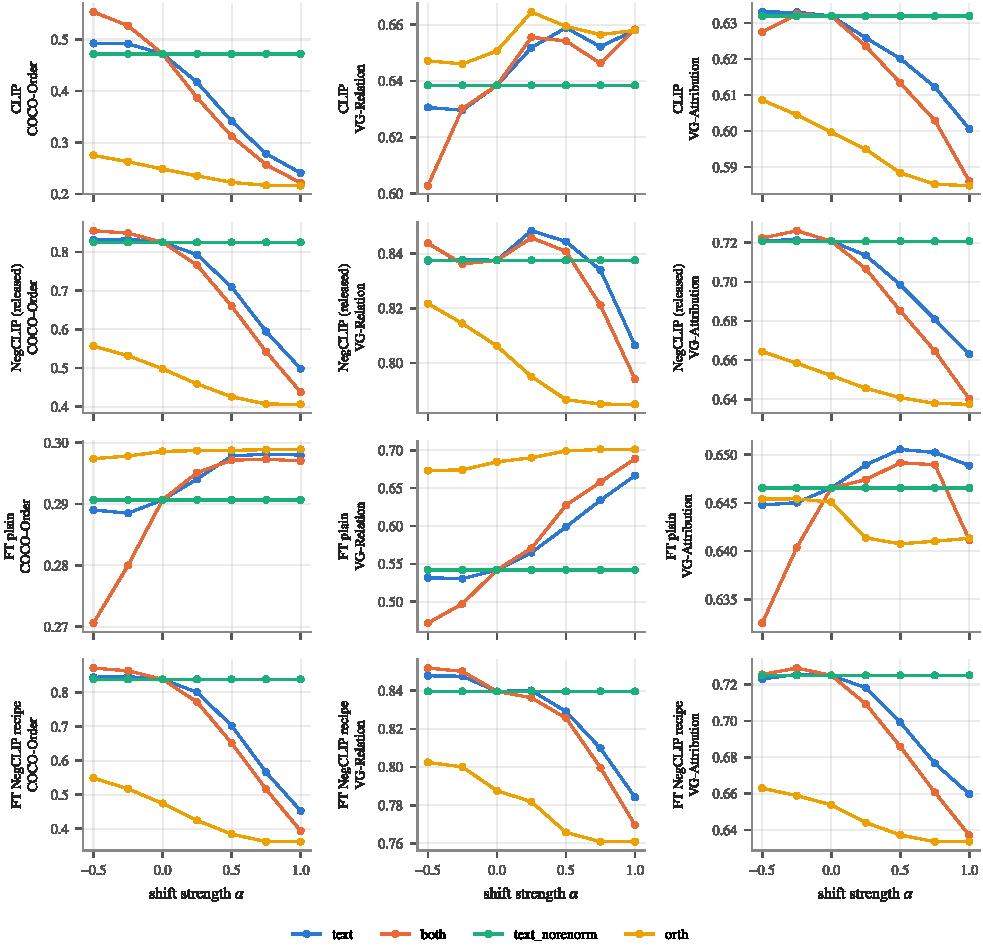
\includegraphics[width=0.92\textwidth]{figs/app_shift_modes}}
\caption{Accuracy against $\alpha$ for the four shift modes on four models. \emph{text\_norenorm} is flat. \emph{orth} starts lower at $\alpha=0$ because it already removes the deviation along $\uhat$, and then changes much less than the other modes.}
\label{fig:app_modes}
\end{center}
\end{figure}

\textbf{Floating-point ties.} In exact arithmetic \emph{norenorm} cannot change any ranking. In float32 a handful of near-ties (caption scores equal to about seven decimals) can flip when a large constant is added; on COCO-Order this happens in 2 of 25,010 cases for CLIP, below the fourth decimal of accuracy.

\section{Learning Rate and Post-Hoc Closing}
\label{app:lr}

Each of the 30 grid runs was encoded and shifted to a remaining gap of 0.10 with the text shift, and separately had its deviation $d$ along $\uhat$ removed (\emph{orth}, $\alpha{=}0$). \Cref{tab:lr} gives the changes averaged over the available seeds; \cref{fig:lr} plots them.

\begin{table}[H]
\caption{Accuracy change for every grid run, averaged over $n$ seeds. gap: $\gapnorm$ on COCO val before the shift. close: text shift to a remaining gap of 0.10. rem.\ $d$: removal of $d$ only. Abbreviations as in \cref{tab:matched}.}
\label{tab:lr}
\begin{center}
\begin{small}
\begin{tabular}{llcccccccc}
\toprule
& & & & \multicolumn{2}{c}{COCO-Order} & VG-Relation & VG-Attribution & R@1 \\
Configuration & lr & $n$ & gap & close & rem.\ $d$ & close & close & close \\
\midrule
\csname @@input\endcsname lr_table.tex
\bottomrule
\end{tabular}
\end{small}
\end{center}
\end{table}

\section{SugarCrepe}
\label{app:sugarcrepe}

\begin{figure}[H]
\begin{center}
\centerline{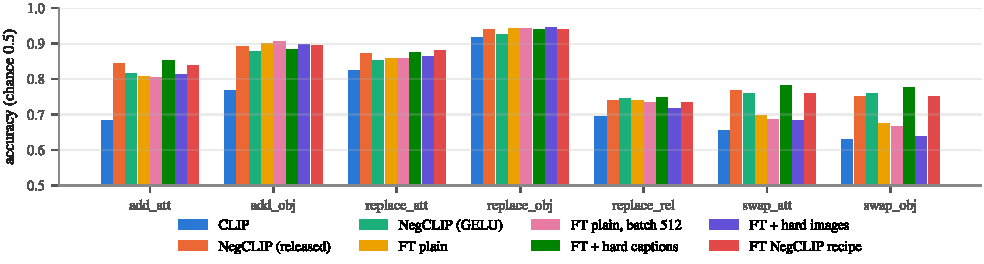
\includegraphics[width=\textwidth]{figs/app_sugarcrepe_clean}}
\caption{Clean SugarCrepe accuracy per subset.}
\label{fig:app_sc}
\end{center}
\end{figure}

\begin{table}[H]
\caption{Clean SugarCrepe accuracy per subset and mean over subsets.}
\label{tab:sc}
\begin{center}
\begin{small}
\begin{tabular}{lcccccccc}
\toprule
Model & add-att & add-obj & replace-att & replace-obj & replace-rel & swap-att & swap-obj & mean \\
\midrule
CLIP & 0.684 & 0.767 & 0.824 & 0.918 & 0.695 & 0.655 & 0.629 & 0.739 \\
NegCLIP (released) & 0.844 & 0.892 & 0.873 & 0.939 & 0.739 & 0.767 & 0.751 & 0.829 \\
NegCLIP (GELU) & 0.815 & 0.879 & 0.852 & 0.926 & 0.746 & 0.758 & 0.759 & 0.819 \\
FT plain & 0.806 & 0.900 & 0.859 & 0.942 & 0.740 & 0.697 & 0.673 & 0.803 \\
FT plain, batch 512 & 0.805 & 0.906 & 0.858 & 0.942 & 0.735 & 0.686 & 0.665 & 0.800 \\
FT + hard captions & \textbf{0.851} & 0.884 & 0.876 & 0.941 & \textbf{0.748} & \textbf{0.782} & \textbf{0.776} & \textbf{0.837} \\
FT + hard images & 0.812 & 0.897 & 0.863 & \textbf{0.946} & 0.718 & 0.682 & 0.637 & 0.793 \\
FT NegCLIP recipe & 0.838 & 0.894 & \textbf{0.879} & 0.938 & 0.733 & 0.760 & 0.751 & 0.828 \\
\bottomrule
\end{tabular}
\end{small}
\end{center}
\end{table}

Plain COCO fine-tuning already lifts the add and replace subsets; only hard captions lift the swap subsets, and hard images add nothing there. After closing the gap, replace-obj does not move for any model. The gains of the add subsets after closing the gap are analysed in \cref{sec:exp} together with caption length.

\section{Robustness to Embedding Noise}
\label{app:noise}

\begin{figure}[H]
\begin{center}
\centerline{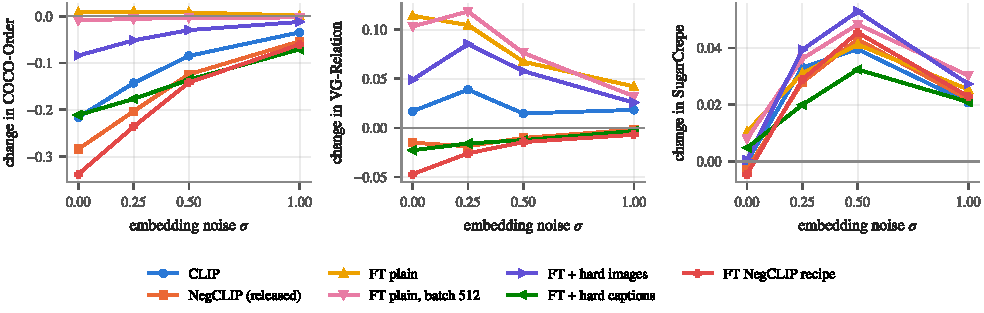
\includegraphics[width=\textwidth]{figs/app_noise}}
\caption{Change in accuracy from closing the gap (to 0.10) at each noise level $\sigma$ (mean of 3 noise seeds).}
\label{fig:app_noise}
\end{center}
\end{figure}



\section{Additional Analyses of the Gap Direction}
\label{app:extra}

The removal operation used throughout is the \emph{orth} control at $\alpha=0$: each caption's deviation from the benchmark mean along a direction (or inside a subspace) is removed and the embedding is re-normalised. \Cref{tab:x_auc} gives the one-coordinate probe for every model and benchmark, and \cref{tab:x_keep} the deviation-preserving variant of the text shift.

\begin{table}[H]
\caption{Probability that the true caption has a larger coordinate along $\uhat$ than a negative caption of the same case (0.5 = no information).}
\label{tab:x_auc}
\begin{center}
\begin{small}
\begin{tabular}{lcccc}
\toprule
Model & COCO-Order & VG-Relation & VG-Attribution & SugarCrepe \\
\midrule
CLIP & 0.679 & 0.483 & 0.516 & 0.412 \\
NegCLIP (released) & 0.791 & 0.549 & 0.583 & 0.372 \\
NegCLIP (GELU) & 0.770 & 0.523 & 0.555 & 0.373 \\
FT plain & 0.425 & 0.430 & 0.461 & 0.337 \\
FT plain, batch 512 & 0.457 & 0.429 & 0.469 & 0.330 \\
FT + hard captions & 0.828 & 0.558 & 0.614 & 0.373 \\
FT + hard images & 0.557 & 0.457 & 0.509 & 0.353 \\
FT NegCLIP recipe & 0.819 & 0.558 & 0.585 & 0.382 \\
\bottomrule
\end{tabular}
\end{small}
\end{center}
\end{table}

\begin{table}[H]
\caption{Closing the gap to 0.10 with the text shift, and with the deviation along $\uhat$ restored (``keep $d$''), clean and at noise $\sigma=0.5$ (3 noise seeds).}
\label{tab:x_keep}
\begin{center}
\begin{small}
\begin{tabular}{lccccccc}
\toprule
& & \multicolumn{3}{c}{COCO-Order} & \multicolumn{3}{c}{COCO text$\to$image R@1} \\
Model & $\sigma$ & no shift & text shift & keep $d$ & no shift & text shift & keep $d$ \\
\midrule
CLIP & 0 & 0.472 & 0.256 & 0.268 & 0.302 & 0.198 & 0.197 \\
 & 0.5 & 0.320 & 0.239 & 0.246 & 0.158 & 0.130 & 0.130 \\
NegCLIP (released) & 0 & 0.825 & 0.541 & 0.579 & 0.448 & 0.358 & 0.358 \\
 & 0.5 & 0.532 & 0.408 & 0.426 & 0.279 & 0.254 & 0.253 \\
FT plain & 0 & 0.291 & 0.299 & 0.296 & 0.454 & 0.384 & 0.384 \\
 & 0.5 & 0.251 & 0.259 & 0.257 & 0.319 & 0.288 & 0.287 \\
FT + hard captions & 0 & 0.878 & 0.667 & 0.704 & 0.454 & 0.389 & 0.390 \\
 & 0.5 & 0.649 & 0.515 & 0.536 & 0.325 & 0.298 & 0.298 \\
FT NegCLIP recipe & 0 & 0.838 & 0.501 & 0.546 & 0.449 & 0.351 & 0.351 \\
 & 0.5 & 0.514 & 0.372 & 0.392 & 0.267 & 0.243 & 0.242 \\
\bottomrule
\end{tabular}
\end{small}
\end{center}
\end{table}

\section{Closing the Gap During Training}
\label{app:gapreg}

The penalty $\lambda\lVert\frac{1}{n}\sum_i x_i-\frac{1}{n}\sum_i y_i\rVert^2$ is computed on each batch over the images and their matched captions (hard negative captions are excluded) and added to the loss of \cref{eq:loss}. All other settings are those of the main grid (lr $5{\times}10^{-6}$, seed 0, 5 epochs). \Cref{fig:x_gapreg} shows the validation gap during training. The gap measured on all 25,010 COCO-val captions after training is 0.04--0.05. Validation mean Recall@1 at the end of training is 0.413--0.439, against 0.420--0.457 for the same configurations without the penalty.

In the regularised models the gap direction no longer carries compositional information: removing each caption's deviation along $\uhat$ changes COCO-Order by at most 0.009 and VG-Relation by at most 0.038, and the probe value for COCO-Order is 0.35--0.79 without a consistent sign. Closing the gap during training does not improve robustness to embedding noise: at $\sigma=0.5$, COCO text$\to$image Recall@1 is 0.301 for FT + hard captions with $\lambda=10$ against 0.322 without the penalty, and 0.298 against 0.317 for FT plain. These runs use a single seed; the COCO-Order gains for the hard-caption configurations (0.03--0.08) are 5--10 times the seed standard deviation of \cref{tab:matched}.

\section{Caption Naturalness}
\label{app:nat}

In our mid-project analysis, word-shuffled COCO-Order captions tended to lie further on the text side of $\uhat$ than the true captions, which suggested that $\uhat$ might encode how natural a caption reads. We tested this with GPT-2 small: for each of the 119,724 COCO-Order captions (true and shuffled) we computed its perplexity and its projection $y^\top\uhat$, and measured the Spearman correlation per model (\cref{fig:app_nat}, \cref{tab:nat}). All correlations are below 0.2 in magnitude and change sign between models. They are somewhat stronger for hard-caption models ($-0.18$, $-0.15$, $-0.12$), but far too weak for $\uhat$ to be a naturalness direction.

\begin{figure}[H]
\begin{center}
\centerline{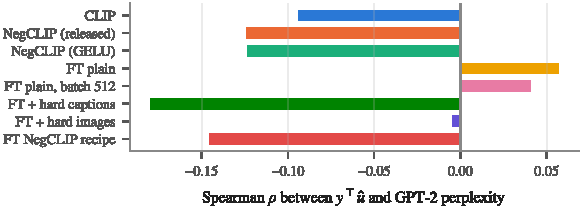
\includegraphics[width=0.55\textwidth]{figs/app_naturalness}}
\caption{Spearman correlation between each COCO-Order caption's projection on $\uhat$ and its GPT-2 perplexity.}
\label{fig:app_nat}
\end{center}
\end{figure}

\begin{table}[H]
\caption{Spearman $\rho$ between $y^\top\uhat$ and GPT-2 perplexity ($n=119{,}724$; all $p<10^{-30}$ except FT + hard images, $p=0.14$).}
\label{tab:nat}
\begin{center}
\begin{small}
\begin{tabular}{lcccccccc}
\toprule
& CLIP & NegCLIP & NegCLIP (GELU) & FT plain & FT 512 & FT + cap. & FT + img. & FT NegCLIP \\
\midrule
$\rho$ & $-0.094$ & $-0.124$ & $-0.124$ & $+0.057$ & $+0.041$ & $-0.180$ & $-0.004$ & $-0.146$ \\
\bottomrule
\end{tabular}
\end{small}
\end{center}
\end{table}

\section{Summary of Findings}
\label{app:summary}

\begin{table}[H]
\caption{Hypotheses and the main evidence for each outcome. C-Ord: COCO-Order; R@1: COCO image$\to$text Recall@1.}
\label{tab:summary}
\begin{center}
\begin{small}
\begin{tabular}{@{}>{\raggedright\arraybackslash}p{0.3\textwidth}>{\raggedright\arraybackslash}p{0.66\textwidth}@{}}
\toprule
Hypothesis & Outcome \\
\midrule
H1: hard-negative training changes the gap & Partly supported: hard images shrink it (0.650 vs 0.775 at $5{\times}10^{-6}$); hard captions do not (0.758). \\
H2: closing the gap is free & Rejected on clean data: C-Ord $-0.12$ to $-0.38$ for hard-caption models, R@1 $-0.04$ to $-0.21$; SugarCrepe gains 0.03--0.05 only under noise. \\
H3: a uniform text shift keeps rankings & Holds only without re-normalisation; with it, the shift removes the coordinate $d$. \\
Closing the gap during training & No loss: C-Ord $+0.03$ to $+0.08$ for hard-caption models at a gap of 0.03. \\
\bottomrule
\end{tabular}
\end{small}
\end{center}
\end{table}

\end{document}
